\section{Results \& Discussion}
\label{sec:results}
Because the men would hang around the corner on windy days\cite{dresses}, a windy day was simulated with a wind speed of 9~ms$^{-1}$\footnote{The average windpeed 2~km from the Flatiron building is about 4.5~ms$^{-1}$\cite{windspeed}, so a windy day is approximated as twice the average windspeed.}. To get an accurate simulation, the simulation was ended when it converged to a residual of $10^{-4}$. 

In order to adequately judge the wind around the building, an overview is created by plotting the streamlines at 3 different heights: the bottom(\autoref{fig:streamlinesbottom}), around the middle(\autoref{fig:streamlinesmid}) and at the top(\autoref{fig:streamlinestop}) of the Flatiron building and can be found in \autoref{sec:streamlines}.

To check if women's ankles would really show, a plot of the velocity in the $z-$direction, the pressure and the turbulence kinetic energy were made at a height of 1.37 meter (this was the lowest the program could go). These are shown in \autoref{fig:zvelocity}, \ref{fig:zpressure} and \ref{fig:zenergy} respectively.

\begin{figure}[htp]
\centering
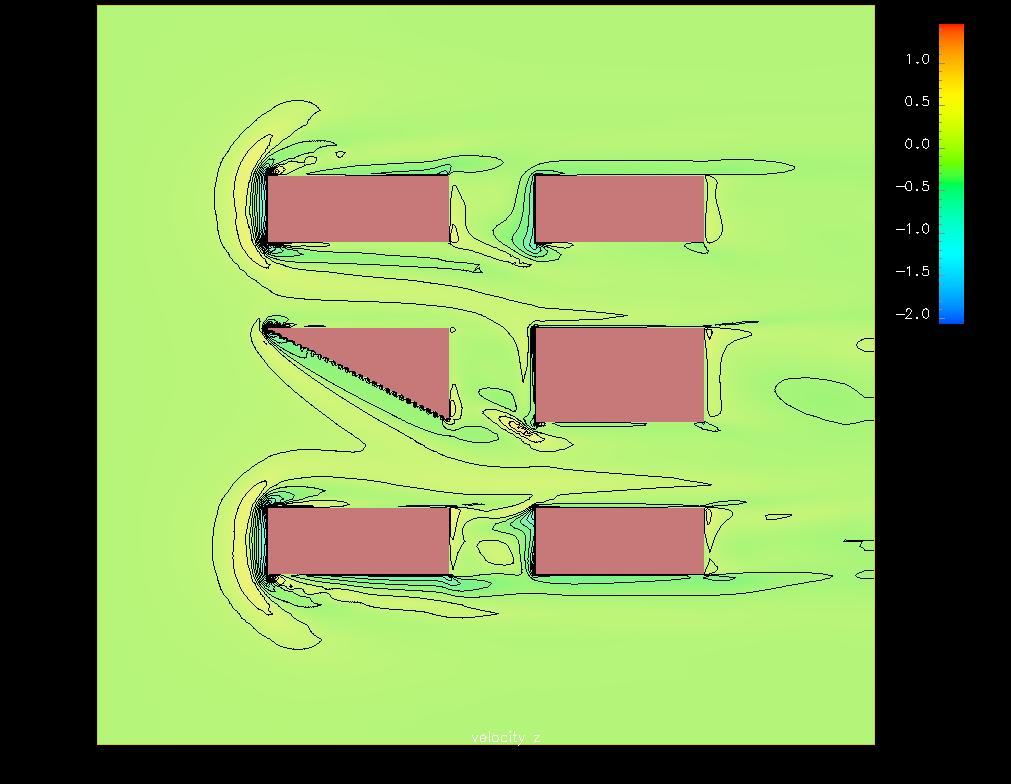
\includegraphics[width = \textwidth]{zvelocity.png}
\caption{Velocity (in ms$^{-1}$)in the $z-$direction around the Flatiron building at $z=1.37$~m}
\label{fig:zvelocity}
\end{figure}
\begin{figure}[htp]
\centering
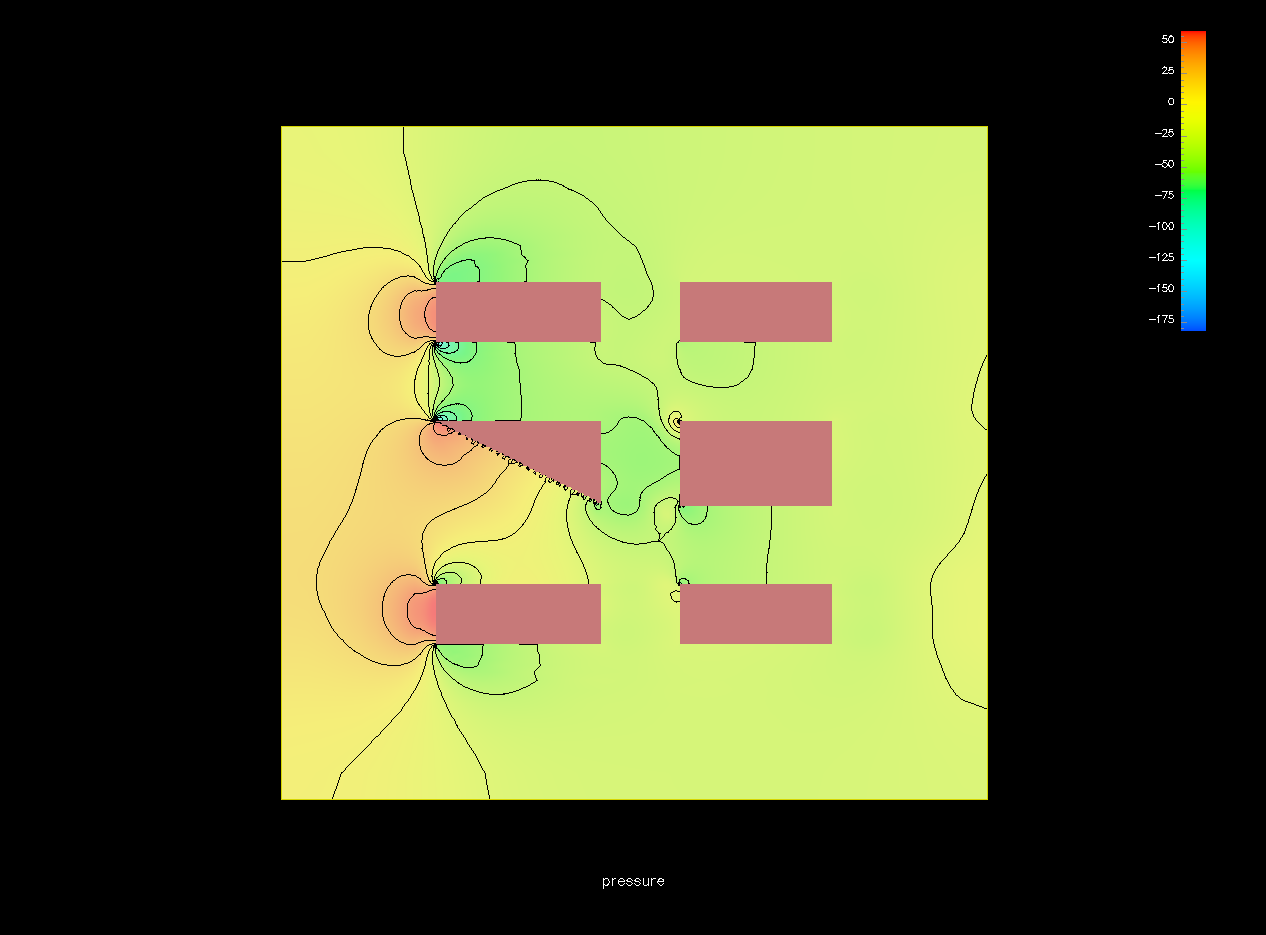
\includegraphics[width = \textwidth]{zpressure.png}
\caption{Pressure distribution(in Pa) around the Flatiron building at $z=1.37$~m}
\label{fig:zpressure}
\end{figure}
\begin{figure}[htp]
\centering
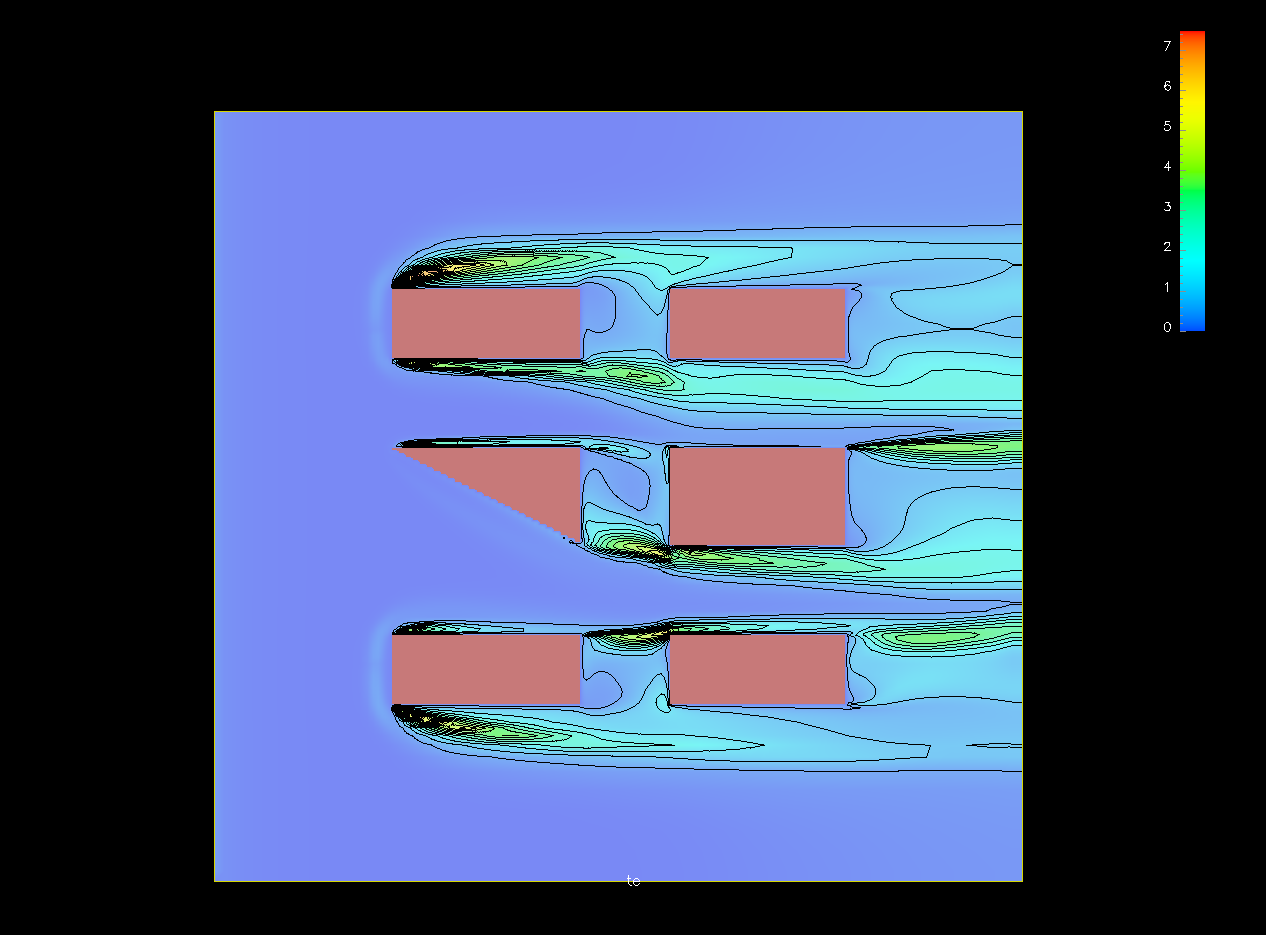
\includegraphics[width = \textwidth]{zenergy.png}
\caption{Turbulence kinetic energy(in m$^2$s$^{-2}$) around the Flatiron building at $z=1.37$~m}
\label{fig:zenergy}
\end{figure}

What is most interesting about the Flatiron building is the way it diverges the air. As seen in \autoref{fig:zenergy}, there is barely any turbulence at the tip of the Flatiron building (a maximum turbulence kinetic energy of $k=2$~m$^2$s$^{-2}$) while at the other most upfront buildings, around the corners there is up to 7~m$^2$s$^{-2}$. The air at the Flatiron building does not have to come to a full stop in the $x-$direction, so there is not an abrupt change of velocity direction. The air still collides with tip of the building, so it is slightly deflected. From \autoref{fig:zpressure} it is visible that the deflected air follows the diagonal side well, while the deflection causes some turbulence at the long straight side. 

At the widest point of the Flatiron building, there is a lot of turbulence kinetic energy. \autoref{fig:streamlinesbottom} shows that some air that flows along the long straight side ducks behind the building into the perpendicular street. The collision of this stream and the stream that flows along the diagonal side is probably the cause of the turbulence in this area. The stream going behind the building is caused by the low pressure area behind the Flatiron building (see \autoref{fig:zpressure}), sucking air into the street. So why isn't any air sucked in from the diagonal stream? In fact, this stream starts with a velocity component in the $y-$direction, but gets bent into the $x-$direction. So it does experience a change in momentum due to the pressure gradient. Since the speed of the diagonal stream is also higher, it does not get sucked into the street, but it does collide with the other stream and the building behind it. This in turn causes a rise in pressure and turbulent energy, which creates a small updraft, seen in \autoref{fig:zvelocity}. 

To see if this updraft is strong enough to blow up women's skirts, a very rough estimation has been made of the how fast the wind has to be blowing upwards to overcome gravity. As the calculations in \autoref{airspeedestimation} show, the wind has to be blowing upwards with a speed of 1.3 ms$^{-1}$ to prove the if the myth is true.